\chapter{Collectivity and Flow in QCD Systems}
\section{A Conceptual Understanding of Collectivity and Flow}
The observation of collectivity in matter can be a powerful indicator of fundamental properties in that matter. Collectivity means many discrete structures are interacting together to form a whole otherwise known as highly correlated behavior. In high energy heavy ion physics, a common interpretation of this behavior, although not the only interpretation\footnote{Although it is common to think of collectivity as hydrodynamic behavior, observations of collectivity do not necessarily imply any specific interpretation. Later we will discuss some alternative interpretations such as glasma correlations.}, is of a locally equilibrated medium with bulk properties instead of a group of individually interacting constituent particles. In this case, the medium would be QGP and the bulk properties would be that of a hydrodynamically described fluid: viscosity, density, temperature, etc. The term collectivity is often synonymous with the term hydrodynamic flow or simply flow. In this thesis, the terms will be used synonymously except in specific cases where the distinction is important.

It is important to note that although collectivity has a distinct signal, there are possible sources that can produce such a signal which do not involve collective behavior. These sources are called ``non-flow" to differentiate them from sources of collectivity, such as flow. Especially true in small collision systems, non-flow is the largest background component when measuring collectivity. Thus, when making measurements, often non-flow must be taken into account as either a systematic uncertainty or as a systematic error correction. Sources of non-flow will be discussed more in Chapter 5 section .xxx. 

To assist in the discussion of flow, we will describe how it is measured briefly. Generally flow can be observed in heavy ion collisions by looking for long-range angular correlations in the spray of final state particles that come out of the collision. ``Long-range angular correlations" in this case refers to correlations in particles with trajectories that have a large separation in pseudorapiditiy $\eta$. When looking for correlations, this separation in $\eta$ ensures that we are measuring something other than just local correlations, which are often due to non-flow. 

Conceptually, the story of flow is that patterns in the initial conditions of the medium will be carried through the medium evolution and observable in the final state particles. Figure \ref{fig:standard_flow_diagram} demonstrates the key events in the story: initial state geometry becomes transformed into a final state momentum anisotropy. The consideration of initial collision geometry will be a reoccurring theme when interpreting results in this thesis because the initial state geometry is one of the few independent variables over which we have experimental control.

\begin{figure}[!ht]
\begin{center}
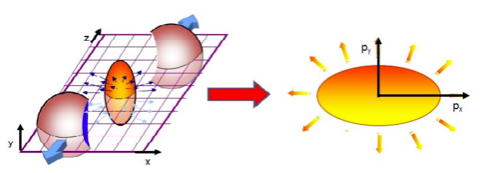
\includegraphics[width=0.55\linewidth]{figs/elliptical_flow_cartoon.png}
\caption{A diagram demonstrating the relation between initial state geometry being transformed into final state momentum anisotropy. The left depicts two spherical nuclei colliding parallel to the z-axis. The pair of nuclei leave behind ellipsoid corresponding to the almond-shaped elliptical overlap region present in the initial state collision geometry. This ellipsoid hydrodynamically evolves such that it expands along the steepest pressure gradient which corresponds to the transverse (x-y plane). The right depicts the elliptical pattern present in transverse momentum distribution of the final state particles after the medium has finished evolving.}
\label{fig:standard_flow_diagram}
\end{center}
\end{figure}

\subsection{Initial Conditions}
Before proceeding in describing flow mathematically, it is useful to talk about the initial conditions of heavy ion collisions. When talking about collisions of spherically symmetric bodies, one of the most relevant parameters in characterizing collisions is known as the impact parameter. The impact parameter is the distance between the center of mass of each collision body, the larger the impact parameter, the more peripheral the collision. For heavy ion collisions, it is useful to consider peripheral collisions along with other types, as shown in Figure \ref{fig:centrality_diagram}. The degree in which the colliding nuclei overlap is known as the ``centrality." A small value for centrality, for example 0-10\%, corresponds to more central collision events, while a large value for centrality, for example 60-100\%, corresponds to more peripheral collisions. The method for quantifying the event's centrality is discussed in Chapter 3.
\begin{figure}[!ht]
\begin{center}
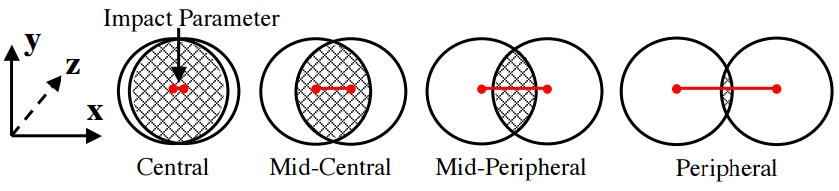
\includegraphics[width=0.55\linewidth]{figs/centrality_impact_parameter_diagram.PNG}
\caption{A diagram of the possible initial conditions of heavy ion collisions. The impact parameter is the red line. The language used in heavy ion physics is as follows: the larger the overlap between the colliding nuclei, the more central it is, the smaller the overlap, the more peripheral it is.}
\label{fig:centrality_diagram}
\end{center}
\end{figure}

%The centrality determination 
%\begin{equation}
%\label{eqn:eccentricity_equation}
%\varepsilon_n = \frac{\sqrt{<r^2 \cos(n\phi)>^2+<r^2 \sin(n\phi)>^2}}{<r^2>},
%\end{equation}


\section{Mathematical Introduction to Measuring and Quantifying Flow}

As discussed above, looking for long-range angular correlations is a way to measure flow. Measuring the azimuthal anisotropy is a way to quantify the extent of long-range angular correlation present in the medium evolution. Azimuthal anisotropy is the degree to which measured particles are non-uniform in the transverse plane. There are a number of ways to measure the azimuthal anisotropy. We will start by creating a correlation function. 

\subsection{Two-Particle Correlations}

A correlation function is dependent on the difference in particles' trajectories, rather than the trajectories of the particles themselves. Let us consider the two-particle correlation function which uses \textbf{pairs} of particles from a collision event in order to create a correlation function. For each each pair in an event, a $\Delta\phi$ = $\phi_1$ - $\phi_2$, and a $\Delta\eta$ = $\eta_1$ - $\eta_2$, value is obtained which makes up the signal $S(\Delta\phi,\Delta\eta)$ for a single event: 

\begin{equation}
  S(\Delta\phi,\Delta\eta) = \sum_{j=1}^{N_{\rm particles}}\left(\sum_{i=j+1}^{N_{\rm particles}}s(\phi_i - \phi_j,\eta_i - \eta_j)\right)=\sum_{k=1}^{N_{\rm pairs}}s(\Delta\phi_k,\Delta\eta_k),
\end{equation}
where $s(\phi_i - \phi_j,\eta_i - \eta_j) = s(\Delta\phi_k,\Delta\eta_k)$ is a single pair in an event, $N_{\rm particles}$ is the number of particles in an event, and $N_{\rm pairs}$ is the number of unique pairs in an event. This pair counting scheme ensures that no pair will be double counted and that a particle can not form a pair with itself.

Ideally, this $S(\Delta\phi,\Delta\eta)$ would be the correlation function; however, there are artificial correlations due to detector acceptance and other sources which would distort this distribution. In order to correct for these effects, a mixed event background distribution $M(\Delta\phi,\Delta\eta)$ is created, whereby pairs are produced by particles from two different events. Then correlation function can be defined as follows:

\begin{equation}
  C(\Delta\phi,\Delta\eta) =
          \frac{S(\Delta\phi,\Delta\eta)}{M(\Delta\phi,\Delta\eta)} 
          \frac{\int M(\Delta\phi,\Delta\eta) \, d\Delta\phi d\Delta\eta}{\int S(\Delta\phi,\Delta\eta) \, d\Delta\phi d\Delta\eta},
  \label{eq:def_corr_function}
\end{equation}
where the integration is over the full $\Delta\phi,\Delta\eta$ range in order to normalize the correlation function. Substantial variations in this $C(\Delta\phi,p_T)$ are usually seen as long-range angular correlations which can be attributed to collectivity.

In practice, correlation functions often combine particles from two variable $p_T$ ranges. The first $p_T$ range is known as the ``trigger particles" and the second range is known as the ``associated" particles. In this scheme, the pair function is $s(\phi_i^t - \phi_j^a,\eta_i^t - \eta_j^a)$ where the $t$ superscript indicates trigger particles with a given $p_T$ range and the $a$ superscript indicates associated particles with a given $p_T$ range. 

An example of two 2-D two-particle correlation functions for $p+p$ at \sqsn = 7 TeV with no multiplicity selection $Pb+Pb$ at \sqsn = 2.76 TeV high multiplicity events is shown in Figure \ref{fig:corr_function_example}. The trigger and associated $p_T$ ranges are given in the figure caption. Plotting the correlation function in terms of both $\Delta\phi$ and $\Delta\eta$ allows one to see the full extent and location of correlations for the collision system. These two correlations were selected to showcase the two extremes of typical correlation functions. 

An important feature in the left plot shows a large amount of correlations at $(\Delta\phi,\Delta\eta)$ = (0,0), which is known as the nearside\footnote{For correlation functions, $\Delta\phi $ $\sim$0 is known as ``nearside" and $\Delta\phi  \sim\pi$ is known as ``awayside."} ``jet peak." As mentioned in Chapter 1, jets are a spray of particle in a cone shape; therefore, the jet peak is at (0,0) because all the particles within the jet have nearly the same trajectory. The jet peak has been truncated for plotting reasons because it is so large. Another important feature is what is known as the ``awayside ridge" or ``awayside jet peak" located at $\pi$ and extending very far in the $\Delta\eta$ variable. This feature arises when back-to-back dijets are produced; all of the particles from one of the jets will be roughly $\pi$ radians apart in trajectory with respect to the other jet and spread out in $\Delta\eta$. Apart from these main features which come from jets and dijets, there are no other sources of systematic correlations between particles for minimum bias $p+p$ events, such that $p+p$ events are taken to be the representation of the non-flow background. Thus, correlation function features present in regular $p+p$ events are taken to be present at some level in the correlation function of every heavy ion collision system.

\begin{figure}[!ht]
\begin{center}
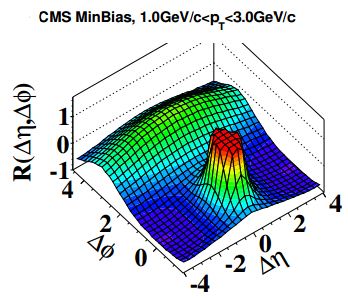
\includegraphics[width=0.43\linewidth]{figs/pp_correlation_function_min_bias.png}
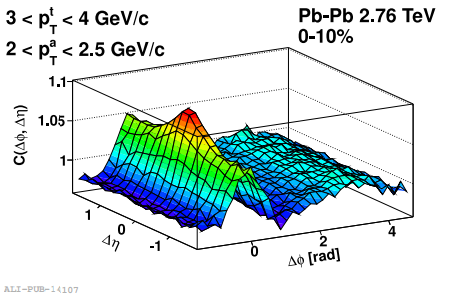
\includegraphics[width=0.48\linewidth]{figs/pbpb_correlation_function_010.png}
\caption{The right plot is 2-D two-particle correlation function for $p+p$ collisions at \sqsn = 7 TeV for hadrons with the same trigger and associated $p_T$ range of 1.0 $<|p_T|<$ 3.0 GeV/c for all events \cite{Khachatryan2010}. The left plot is 2-D two-particle correlation function for $Pb+Pb$ collisions at \sqsn = 2.76 TeV 0-10\%centrality events for trigger hadrons with 3 $<p_T^t<$ 4 GeV/c and associated hadrons with 2 $<p_T^t<$ 2.5 GeV/c measured by ALICE. \textbf{add ref}.}
\label{fig:corr_function_example}
\end{center}
\end{figure}

Conversely, the right panel of \ref{fig:corr_function_example} depicts the correlation function of high multiplicity $Pb+Pb$ events which exhibit characteristics of flow. 
%First of all, the normalization used for this correlation function reveals the magnitude of the deviation in correlations is around 5\%; even with flow present, the magnitude of the bulk effect can be small depending on the initial conditions. Unlike the diagram in Figure \ref{fig:standard_flow_diagram}, the overlap between the spheres is almost total which creates a medium which is nearly azimuthal isotropic. 
While the non-flow features of the nearside jet peak and the awayside peak are present, a new feature known as the ``nearside ridge" is located at $(\Delta\phi,\Delta\eta)$ = (0,$|\Delta\eta|> \sim1.0$). This ridge exists in contrast to the lack of any correlations in the $p+p$ correlation function at that location. It should be noted that the awayside jet ridge has also been modified by the bulk of particles. The nearside ridge and the awayside ridge modification are due to particles with long-range angular correlations. Thus, by quantifying the magnitude of these effects, the degree to which flow is present in the system can be measured.

\subsection{Flow Harmonics}
At this point, it useful to narrow our focus to the region of the correlation function which has long-range angular correlations by taking a projection in $\Delta\phi$ away from the jet peak at $\Delta\eta = 0$. This 1-D two-particle correlation function slice contains the azimuthal anisotropy which should correspond to the degree of flow present in the system. Figure \ref{fig:1d_corr_function_example_fourier} depicts this correlation function $C(\Delta\phi)$ for central $Pb+Pb$ events. In order to quantify the azimuthal anisotropy, $C(\Delta\phi)$ is $\cos$ Fourier expanded:
\begin{equation}\label{eqn:dndphi}
  C(\Delta\phi) \propto 1 + \sum_{n=1}2 v_{n}\cos(n[\Delta\phi]),
\end{equation}
where $v_n$ are known as flow coefficients or flow harmonics and $n$ is the harmonic order. The colored curves in Figure \ref{fig:1d_corr_function_example_fourier} are the first five components of the Fourier decomposition and their amplitudes show their relative strength. The green curve, which peaks at $\Delta\phi = 0$ and $\pi$, corresponds to the second order harmonic, which is related to the second order flow coefficient $v_2$. The reason $v_2$ is singled out is because it corresponds to elliptic flow and because it is the observable measured in this thesis. In order to extract $v_2$ from this, one must calculate $c_2$ defined as:
\begin{equation}
  c_2^{t,a} = \left<\cos(2(\phi_1^t-\phi_2^a)\right>,
\end{equation}
where $\left<\right>$ is defined as the average over each event and all events and where $\phi_1^t$ and $\phi_1^a$ is the trigger and associated particles' $\phi$, respectively. If the trigger and associated particles sets are the same then $\sqrt{c_2}$ = $v_2$; however, if the trigger and associated particle sets are not the same then $c_2^{t,a} $=$v_2^{t}\times v_2^{a}$, where$v_2^{t}$ is the $v_2$ for the set of trigger particles alone and the same with $v_2^a$. This ability to resolve $c_2$ into the two distinct $v_2$ components is only true if factorization holds, which only occurs when the non-flow component of the measurement is small enough.
\begin{figure}[!ht]
\begin{center}
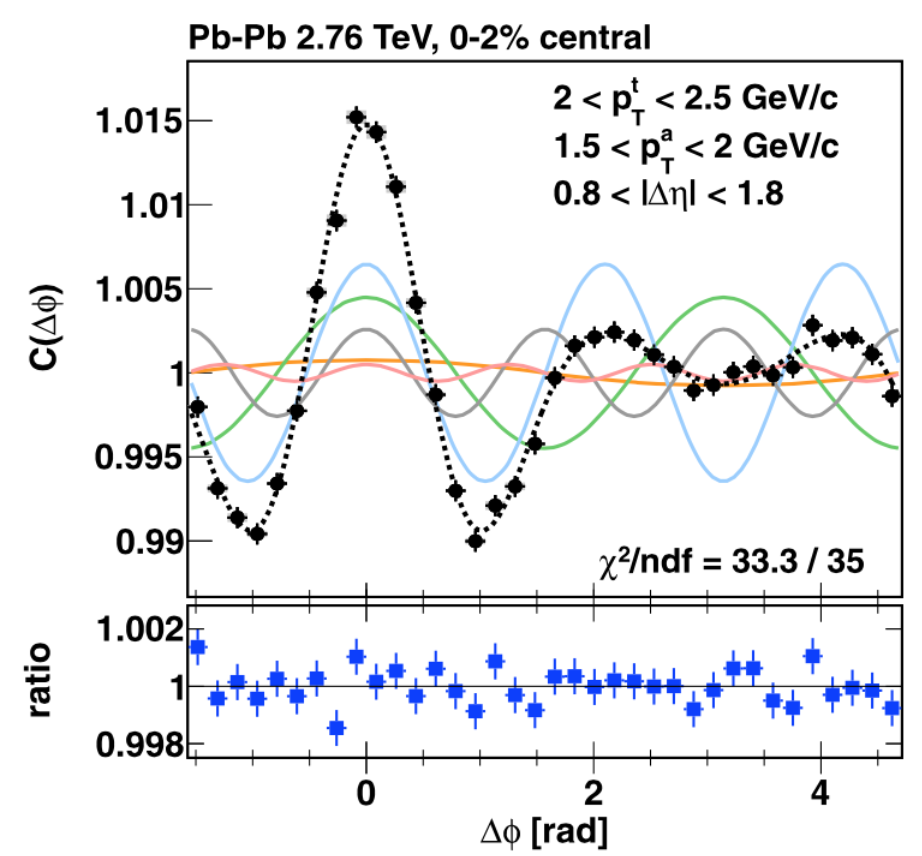
\includegraphics[width=0.48\linewidth]{figs/1d_correlation_function_with_fourier.png}
\caption{The 1-D correlation function in $Pb+Pb$ at \sqsn = 2.76 TeV for the most central events for for trigger hadrons with 2 $<p_T^t<$ 2.5 GeV/c and associated hadrons with 1.5 $<p_T^t<$ 2 GeV/c. The 1-D two-particle correlation function is a projection in $0.8 < |\Delta\eta| < 1.8$ from the 2-D correlation function, the 2-D correlation function being similar to that of the right panel of Figure \ref{fig:corr_function_example}. The black dotted points are the values of the correlation function and the colored lines are the first five $\cos$ Fourier decomposition  components. The black dotted line is the sum of these five components. \textbf{add ref}.}
\label{fig:1d_corr_function_example_fourier}
\end{center}
\end{figure}

\subsection{Cumulants}
Although two-particle correlations are useful, four-particle correlations or more can be used to better understand the flow measurement. In a multi-particle cumulant treatment, $c_n\{k\}$ measures the $n$th harmonic from groups of $k$ particles while explicitly subtracting correlations from $< k$ particles. In this formulation, two-particle cumulants are treated the same way as in two-particle correlation functions:
\begin{equation}
v_2\{2\} = \sqrt{c_2\{2\}} = \sqrt{\left<\cos(2(\phi_1-\phi_2))\right>},
\label{eqn:v22}
\end{equation}
whereas four-particle cumulants are defined as:
\begin{equation}
v_2\{4\} = (-c_2\{4\})^{1/4} =  (2\left<\cos(2(\phi_1-\phi_2))\right>)^2 - \left<\cos(2(\phi_1 + \phi_2 - \phi_3 - \phi_4))\right>)^{1/4},
\label{eqn:v24}
\end{equation}
where the term with four $\phi$ indices corresponds to the four-particle correlation and the term with two $\phi$ indices corresponds to the subtracted off two-particle correlation term. Multi-particle cumulants are well defined for larger groupings of particles, $v_2\{6\}$, $v_2\{8\}$, and up. Comparing $v_2$ measured by two and four-particle cumulants is useful when estimating the level of fluctuations present in the system, something which will be discussed more in Section .xxx.
\subsection{Event Plane Formulation}
Another mathematical treatment for determining flow coefficients involves measuring a mathematical object known as an ``event plane." Conceptually, the event plane method is an attempt to measure the reaction plane angle, which defines the plane to which it is aligned with the orientation of the initial state collision geometry. Figure \ref{fig:reaction_plane_diagram} is a geometric diagram defining the reaction plane angle $\Psi_{RP}$.

\begin{figure}[!ht]
\begin{center}
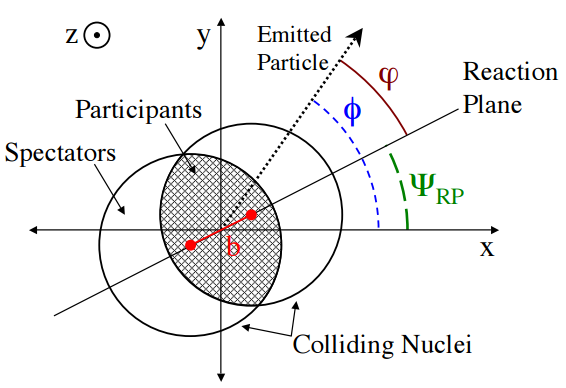
\includegraphics[width=0.68\linewidth]{figs/reaction_plane_diagram.PNG}%from Eric_Richardson_Dissertation fig 1.11
\caption{Diagram showing from the beam’s point of view several variables used to characterize events. The spectators are the nucleons which do not participate in the collision, as opposed to the participants which do participate in the collision. The impact parameter denoted as $b$ and $\Psi_{RP}$ is the reaction or participant plane angle. $\phi$ is the standard azimuthal and $\varphi$ = $\phi$ - $\Psi_{RP}$. \textbf{add ref}}
\label{fig:reaction_plane_diagram}
\end{center}
\end{figure}

The event plane method uses final state particles to calculate the event plane angle from the data. A different event plane angle is defined for each harmonic, and is denoted as $\Psi_n$ where $n$ is the harmonic number. For an event with $N$ particles, define the flow vector $\vec{Q}$ as follows:

\begin{align}
Q_x &= \sum_i^{N}( w_i * \cos(n * \phi_i)) \\
Q_y &= \sum_i^{N}( w_i * \sin(n * \phi_i)) \\
Q_w &= \sum_i^{N}( w_i )
%\Psi_n &= \arctan( \frac{Q_y}{Q_x} ),
\label{eqn:general_ep_math}
\end{align}

where $i$ is the $i$th particle in the event, $\phi_i$ is the azimuthal angle of the particle, $w_i$ is the weight factor, and $n$ is the harmonic number.

We define the $n$th order event plane as
$$\Psi_n = \arctan \left( \frac{Q_y}{Q_x} \right) $$

Once the event plane has been calculated, the flow harmonics ($v_n$) are defined as
\begin{equation}
v_n = \frac{\langle \langle\cos(n(\phi - \Psi_n))\rangle \rangle}{Resolution(\Psi_n)},
\end{equation}

where $\langle \langle \rangle \rangle$ indicates that $\cos(2\phi-\psi)$ is averaged over all particles in the same event, and the resulting $v_2$ must be averaged over many events \cite{PhysRevC.58.1671}. 

The event plane resolution is calculated using the standard 3-sub event method\cite{PhysRevC.58.1671}. The strategy of this method is to measure $\Psi_n$ with three
different detectors in the same event, in order to better constrain the overall measurement of $\Psi_n$. The event plane resolution is defined as
\begin{equation}
Res(\Psi_n^A) = \sqrt{\frac{\left<\cos(n(\Psi_n^A - \Psi_n^B))\right>\left<\cos(n(\Psi_n^A - \Psi_n^C))\right>}{\left<\cos(n(\Psi_n^B - \Psi_n^C))\right>}},
\label{eqn:res}
\end{equation}
where A,B, and C are three detectors measuring the same event. In this context, the term ``sub-event'' refers to the specific subset of particles measured by a given detector, assuming no decorrelation \cite{PhysRevC.58.1671}.

%\begin{equation}\label{eqn:dndphi}
%  C(\Delta\phi) \propto 1 + \sum_{n=1}2 v_{n}\cos(n[\phi-\Psi_n]) 
%\end{equation}
%In order to quantify the azimuthal anisotropy, $C(\Delta\phi,p_T)$ is Fourier transformed:
%\begin{equation}\label{eqn:dndphi}
%  C(\Delta\phi,p_T) \propto 1 + \sum_{n=1}2 v_{n}\cos(n[\phi(p_T)-\Psi_n]) 
%\end{equation}

%\begin{equation}
%\varepsilon_n = \frac{\sqrt{\langle r^2\cos (n\phi)\rangle ^2 + \langle r^2\sin (n\phi) \rangle ^2}}{\langle r^2 \rangle}
%\end{equation}

%\begin{figure}[h!]
%\begin{center}
%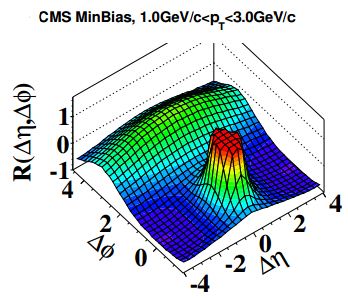
\includegraphics[width=0.45\linewidth]{figs/pp_correlation_function_min_bias.png}
%\caption{ }
%\label{fig:pp_corr_func_minbias}
%\end{center}
%\end{figure}


\section{An Overview of Heavy Ion Models}
Throughout the discovery phase of heavy ion results and beyond, simulations based on theoretical descriptions of heavy ion collisions have been developed and have been successful in describing and predicting results. From the initial state of the colliding nuclei to the final state particles produced, every phase of heavy ion collisions are modeled. First the initial condition models will be discussed and then the medium evolution models will be discussed. It is necessary when calculating observables like $v_n$ to choose an initial state model and a medium evolution model to chain together. The output of the initial state model will be the input to the medium evolution model; therefore, even if the medium evolution model describes the physics well, an initial state model which does not do so would cause the final $v_n$ calculation to be inconsistent with the data. 

%\begin{enumerate}
%\item Initial Collision: 
%\item Pre-equilibrium:
%\item Equilibrated medium Flow
%\item Hadronization and Freeze Out
%\end{enumerate}

\subsection{Initial Condition Models}
Initial condition models use a variety of methods to simulate the colliding nuclei. These models calculate quantities for characterizing initial collision conditions, such as the number of participating nucleons ($N_{part}$), the impact parameter ($b$), and the participant eccentricity ($\varepsilon$). The $N_{part}$ is thought to be related to the size of the medium produced. The $\varepsilon_n$ categorizations the $n$th order anisotropy symmetry in the initial collision geometry which is given by:

\begin{equation}
\label{eqn:eccentricity_equation_ch2}
\varepsilon_n = \frac{\sqrt{<r^2 \cos(n\phi)>^2+<r^2 \sin(n\phi)>^2}}{<r^2>}
\end{equation}
where $r$ is the radius of the participant nucleon. This quantity is important because $v_n \propto \varepsilon_n$ is true in ideal hydrodynamics.

A key part in simulating initial conditions of heavy ion collisions is understanding event-to-event fluctuations.  An important source of fluctuations, generic to all models of quantum fluctuations, are fluctuations in the distributions of nucleons in the nuclear wavefunctions. In addition, there are fluctuations in the color charge distributions inside a nucleon. This, combined with Lorentz contraction, results in “lumpy” transverse projections of color charge configurations that vary event to event. The scale of this lumpiness is given on average by the nuclear saturation scale $Q_s$ which corresponds to distance scales smaller than the nucleon size . For each such configuration of color charges, the Quantum Chromo-Dynamics (QCD) parton model predicts dynamical event-by-event fluctuations in the multiplicities, the impact parameters and the rapidities of produced gluons \cite{PhysRevLett.108.252301}.

\subsubsection{Monte-Carlo Glauber}
There are two main Glauber models: the so called ``optical" Glauber model which assumes a smooth density described by a Fermi distribution in the radial direction; and the Monte-Carlo-based Glauber model where individual nucleons are stochastically distributed on an event basis and collision properties are determined by averaging over multiple events. The optical form of Glauber does not locate nucleons at specific spatial coordinates like the Monte Carlo form of Glauber. While both models give consistent results for determining simple quantities such as $N_{part}$ and $b$, the more statistical Monte-Carlo approach has given $\varepsilon_n$ values that have better agreed with the data. One benefit of the Monte-Carlo approach for quantities like $N_{part}$ is its simplicity and ability to simultaneously simulate experimentally observable quantities, such as charged particle multiplicity. 

The Monte-Carlo Glauber (MC Glauber) model calculation is performed in two steps. At first, the nucleon positions in each nucleus are stochastically determined. Then, the two nuclei are “collided”, assuming the nucleons travel in a straight line along the beam axis (known as the Eikonal approximation), such that nucleons are tagged as wounded (participating) or spectator.

The position of each nucleon in the nucleus is determined according to a probability density function. In a quantum mechanical picture, the probability density function can be thought of as the single-particle probability density and the position as the result of a position measurement. In the determination of the nucleon positions in a given nucleus, it is possible to require a minimum inter-nucleon separation ($d_{min}$) between the centers of the nucleons.

The probability distribution is typically taken to be uniform in azimuthal and polar angles. The radial probability function is modeled from nuclear charge densities extracted in low-energy electron scattering experiments [3]. The nuclear charge density is usually parameterized by a Fermi distribution with three parameters:

\begin{equation}
\rho(r) = \rho_0\frac{1+w(r/R)^2}{1+exp(\frac{r-R}{a})}
\end{equation}
where $\rho_0$ is the nucleon density, $R$ is the radius of the nucleus, $a$ is the skin depth, and $w$ corresponds to deviations from a spherical shape. 

The impact parameter of the collision is chosen randomly from a distribution dN/db $\propto b$ up to some large maximum bmax with bmax 20 fm $>$ 2RA. The centers of the nuclei are calculated and shifted to (-b/2, 0, 0) and (b/2, 0, 0). It is assumed that the nucleons move along a straight trajectory along the beam axis. (The longitudinal coordinate does not play a role in the calculation.) The inelastic nucleon-nucleon cross section ($\sigma_{NN}$), which is only a function of the collision energy is extracted from p+p collisions. At the top RHIC energy of \sqsn = 200 GeV, $\sigma_{NN}$ = 42 mb, while at the LHC it is expected to be around $\sigma_{NN}$ = 72 mb (with large uncertainty from the unknown elastic cross section). The “ball diameter” is defined as:
\begin{equation}
D = \sqrt{\frac{\sigma_{NN}}{\pi}}
\end{equation}
Two nucleons from different nuclei are assumed to collide if their relative transverse distance is less than the ball diameter. If no such nucleon-nucleon collision is registered for any pair of nucleons, then no nucleus-nucleus collision occurred. Counters for determination of the total (geometric) cross section are updated accordingly. An example Au+Au collision event is show in Figure \ref{fig:glauberauauexample}. In this thesis, MC Glauber combined with the negative binomial distribution is used to match the charged particle multiplicity distribution in order to map $N_{part}$ to centrality classes. Details for this procedure are given in Chapter 3, Section xxx.

As stated earlier, and important initial condition quantity in simulating flow is the $\varepsilon$ of the event. MC Glauber simply calculates the moments of the participants themselves for each event. The eccentricity can be calculated along the axis of the participant distribution $\varepsilon_{part}$:
\begin{equation}
\varepsilon_{part} = \frac{\sqrt{(\sigma_x^2-\sigma_y^2)^2+4(\sigma_{xy}^2)^2)}}{\sigma_x^2-\sigma_y^2}
\end{equation}
where $\sigma_{x,y}^2$ are the $x$ and $y$ variances for participating nucleons and $\sigma_{xy}$ is the covariance of $x$ and $y$ for pariticipating nucleons.

\begin{figure}[h!]
\begin{center}
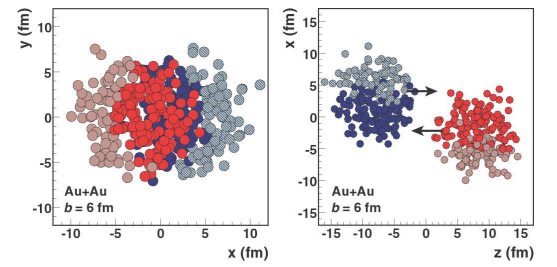
\includegraphics[width=0.65\linewidth]{figs/glauber_auau_example.png}
\caption{Glauber Monte Carlo event (Au+Au \sqsn = 200 GeV with impact parameter $b$ = 6 fm) viewed in the transverse panel and alone the beam axis in the left and right panels, respectively. The deeper color disks correspond to the participating nucleons. \cite{annurev.nucl.57.090506.123020}.}
\label{fig:glauberauauexample}
\end{center}
\end{figure}

%\begin{figure}[h!]
%\begin{center}
%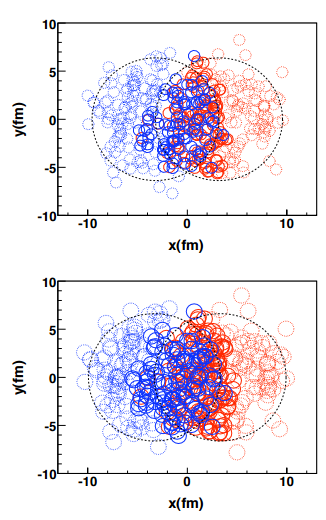
\includegraphics[width=0.45\linewidth]{figs/glauber_auau_pbpb_example.png}
%\caption{Typical events for Au+Au and Pb+Pb collisions which correspond to the top and bottom panels, respectively. The Au+Au calculation was performed at a RHIC energy and the Pb+Pb calculation was at LHC energies. The solid line circles correspond to the participating nucleons while the dotted line circles correspond to the spectators \cite{annurev.nucl.57.090506.123020}.}
%\end{center}
%\end{figure}

%\begin{figure}[h!]
%\begin{center}
%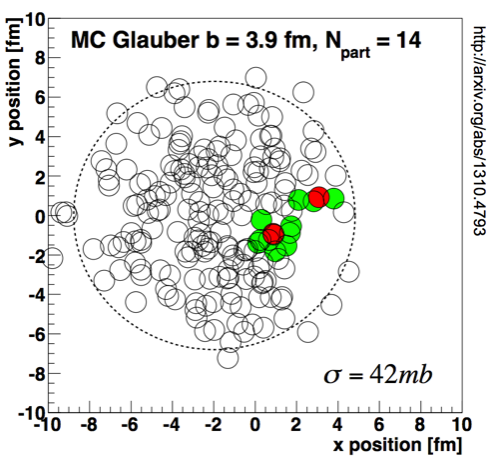
\includegraphics[width=0.45\linewidth]{figs/glauber_event_display.png}
%\caption{}
%\end{center}
%\end{figure}

\subsubsection{IP-Glasma}

Another initial state model is known as IP-Glasma. This model calculates the initial conditions within a Color Glass Condensate (CGC) framework by combining the impact parameter dependent saturation model (IP-Sat) with the Classical Yang-Mills (CYM) description of initial Glasma fields. Calculating initial state dynamics by flowing Glasma gluon fields is thought to be an \textit{ab initio}, or from first principles, approach, although some of the parameters of the model are fixed by diffractive e+p DIS data. The IP-Glasma computation starts by sampling the positions of the constituent nucleons from a Fermi distribution. Then the saturation scale $Q^2_{s,(p)}(x,\textbf{b})$ is obtained from IP-Sat dipole cross section for each nucleus, where $b$ is the impact parameter relative to each participant nucleon's center. Once the saturation scale and the color charge density are obtained, random color charges are sampled from a transverse lattice \cite{PhysRevLett.108.252301}.

A benefit of the IP-Glasma model is that it explicitly includes multiple types of quantum fluctuations, including fluctuations of color charges within the nucleons. It is useful to compare the calculations of IP-Glasma to MC-Glauber in order to gain a greater understanding of both.
\subsubsection{Comparison between IP-Glasma and MC-Glauber}
Figure \ref{fig:ipg_mcg_comp} depict the energy density distributions calculated by the IP-Glasma and MC-Glauber models. It is apparent from the ``lumpiness" of both of these distribution that these models capture the complex internal structure of the nuclei at the moment of collision. However, the MC-Glauber distribution is much smoother than the IP-Glasma distribution due to the fact that the IP-Glasma distribution incorporates fluctuations at a much finer length-scale, given by $1/Q_s(x)$, which creates the spikey structures in the energy distribution. Apart from the differences in the length-scale of fluctuations between the models, MC-Glauber includes the energy distribution from every participant nucleon in the collision event, no matter how glancing its individual collision is, with the same parameters of width. Thus, the MC-Glauber model's procedure for incorporating participating nucleons is less sophisticated than a model like IP-Glasma. However, MC-Glauber has been the most reliable model for providing initial conditions into hydrodynamic models to produce the best results. Although the exact reason for this is unknown, part of the reason should be attributed to the MC-Glauber model's fine tuning to the data. For example, the width of a nucleon's energy density has been chosen to be 0.4 fm for all nucleons to match the MC-Glauber model to the data, despite the fact there are no \textit{ab initio} calculations which derive such a number.

\begin{figure}[h!]
\begin{center}
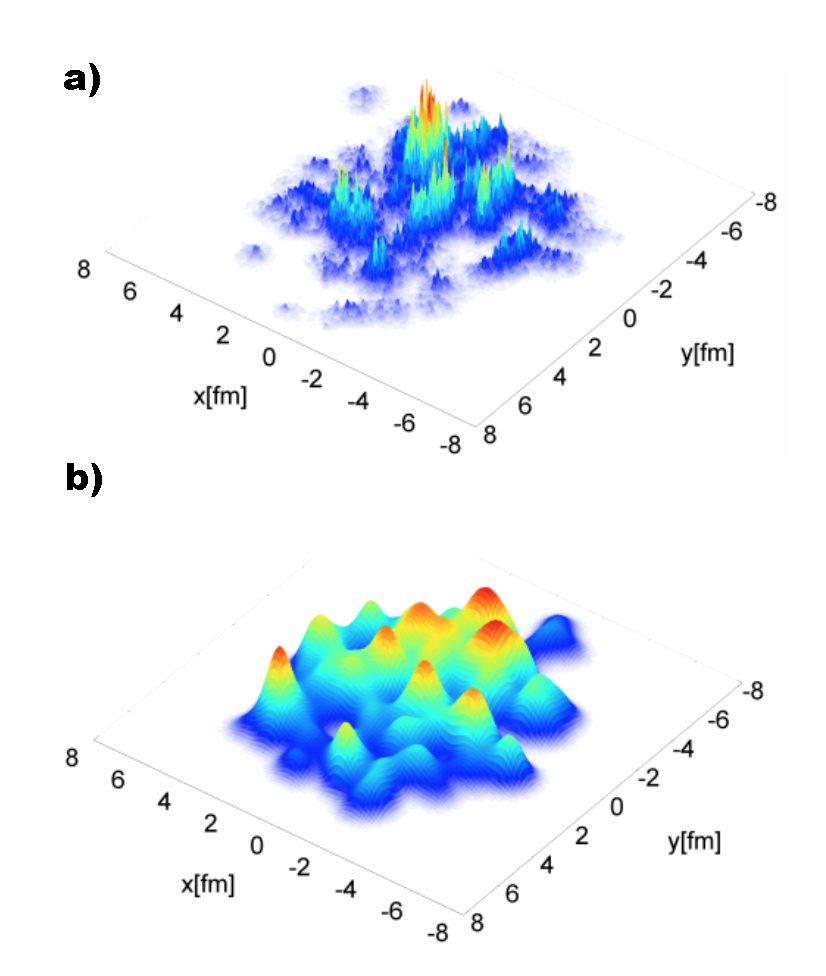
\includegraphics[width=0.45\linewidth]{figs/initial_conditions.png}
\caption{ Initial energy density distributions (arbitrary units) in the transverse plane in two different heavy-ion collision events for IP-glasma  MC-Glauber models in the top and bottom panels, respectively \cite{PhysRevLett.108.252301}.}
\label{fig:ipg_mcg_comp}
\end{center}
\end{figure}

\subsection{Medium Evolution Models}
Once an energy density distribution is calculated from the initial condition models, it used as the input to a medium evolution model. The most commonly used medium evolution model is the relativistic hydrodynamic model treatment.

\subsubsection{Hydrodynamic Modeling}
Relativistic hydrodynamics is a macroscopic tool to simulate the evolution of a strongly coupled QGP medium. It is based on the foundational physical principles of conservation of energy, momentum, and net charge current which are written as:
\begin{align}
\delta_{\mu} T^{\mu\nu}(x) &= 0,\\
\delta_{\mu} N^{\mu}(x) &= 0,
\end{align}
where $T^{\mu\nu}$ is the energy momentum tensor and $N^{\mu}$ is the net baryon charge current. Ideal hydrodynamics requires that the medium is locally equilibrated, such that we have the perfect fluid energy momentum tensor as $T^{\mu\nu} = (e+p)u^\mu u^\nu+pg^{\mu\nu}$ where $e$ is the relativistic rest energy density, $p$ is the fluid pressure, $g^{\mu\nu}$ is the Minkowski metric, and $u^\mu$ is the four-velocity of fluid. Also, the charge current becomes $N^\mu = nu^\mu$ where $n$ is the net baryon density. After asserting an equation of state (EoS) $p = p(n,e)$, the system is closed and the equations can be solved numerically.

Viscous hydrodynamics is similar to ideal hydrodynamics except that viscous hydrodynamics applies to a wider variety of systems, such as imperfectly locally equilibrated systems. In order to account for the lack of equilibrium, several new variables must be introduced: $\pi^{\mu\nu}$ is the sheer stress tensor, $\Pi$ is the bulk pressure, $\eta$ is the sheer viscosity, $\zeta$ is the bulk viscosity, $V^\mu$ is the baryon flow, and $\tau_\pi$ and $\tau_\Pi$ are the corresponding relaxation times. At RHIC and LHC energies, the net baryon density $n$ is zero and $v^\mu$ is assumed to be zero. By choosing a proper EoS, an initial flow velocity, and an initial entropy/energy density at time $\tau_0$, the medium evolution can be simulated for time $\tau > \tau_0$. Note that in order to simulate very early stages during the QGP formation, modifications to this hydrodynamic formulation must account for pre-equilibrium conditions\cite{Song2015}. An example of a hydrodynamic evolution is shown in Figure \ref{fig:heau_sim_evolve}.

To obtain final hadrons, pure hydrodynamic simulations assume free hadron resonances directly emit from the fluid along a decoupling surface. The Cooper-Frye formula [56] is then implemented to calculate the particle momentum distributions, which is followed by a resonance delay routine to generate final stable hadrons. The decoupling surface can be defined by a constant temperature or energy density or other kinetic variables[4, 7]. For the scenario of constant temperature decoupling, $T_dec$ is generally set to 100-130 MeV, depending on the EoS and other hydrodynamic inputs, to allow for sufficient evolution time to build up enough radial flow to fit the slopes of the pT spectra [4].

To simplify numerical simulations, many viscous hydrodynamic calculations assume a specific velocity profile vz = z/t along the beam directions (Bjorken approximation). This leads to a longitudinal boost invariance and reduces the (3+1)-d hydrodynamics to (2+1)-d hydrodynamics. A comparison between the (2+1)-d and (3+1)-d codes has shown that the realistic longitudinal expansion only slightly affects the flow profiles at mid-rapidity [63]. One can still safely investigate the soft particle physics at mid-rapidity using a (2+1)-d code.

\begin{figure}[h!]
\begin{center}
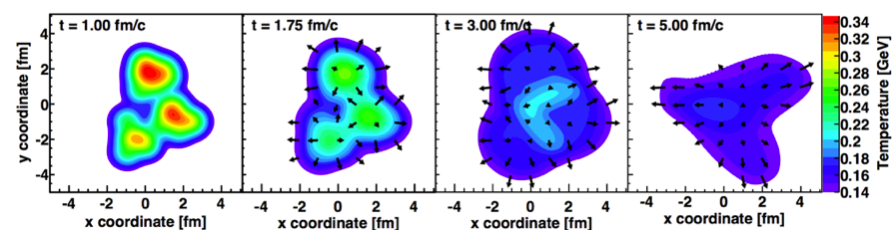
\includegraphics[width=0.69\linewidth]{figs/he3au_simulation.png}
\caption{An example time evolution of a $\hau$ event from the initial state to final state. The color scale indicates the local temperature and the arrows are proportional to the velocity of the fluid cell from which the arrow originates \cite{PhysRevLett.113.112301}.}
\label{fig:heau_sim_evolve}
\end{center}
\end{figure}

\subsubsection{Hybrid Models: SONIC and superSONIC}
A hybrid model matches hydrodynamic descriptions of the expanding QGP to microscopic Boltzmann simulations of the evolving hadronic matter. The transition between models is realized by a Monte-Carlo event generator, which transforms the hydrodynamic output into individual hadrons for succeeding hadron cascade propagations. 

The ``Super hybrid mOdel simulatioN for relativistic heavy-Ion Collisions" (SONIC) combines pre-equilibrium dynamics with hydrodynamics [2] and a late-stage hadronic cascade [3]. In effect, SONIC has only a limited number of parameters, namely those specifying the properties of the incoming nuclei, the speed of sound, and shear and bulk viscosities in the quark–gluon plasma. SONIC is a single shot simulation which obtains a smooth initial condition by averaging large numbers of events and then using that smooth initial condition for one hydrodynamic simulation \cite{Habich:2014jna}.

As discussed when describing initial conditions models, fluctuations play a large role in determining the hydrodynamic flow. In order to study the effects of fluctuations in simulation, an event-by-event simulation is created by inputing fluctuating initial conditions, evolving each system separately, and then averaging the results. This is the motivation behind the development of superSONIC, which is an event-by-event generalization of the SONIC model \cite{Romatschke2015}. Additionally, superSONIC differs from SONIC by incorporating pre-equilibrium dynamics with a calculation in the framework of the AdS/CFT correspondence. The SONIC and superSONIC models agree well with the data within uncertainties.
\subsection{AMPT}
A Multi-Phase Transport (AMPT) model combines partonic and hadronic scattering in a single model. AMPT consists of four main components: the initial conditions, partonic interactions, the conversion from the partonic to the hadronic matter, and hadronic interactions. AMPT uses the Heavy Ion Jet Interaction Generator (HIJING) for generating the initial conditions, Zhang’s Parton Cascade (ZPC) for modeling partonic scatterings, the Lund string fragmentation model or a quark coalescence model for hadronization, and A Relativistic Transport (ART) model for treating hadronic scatterings.
It consists mainly of four components: the HIJING model to convert the initial incident energy to the production of hard minijet partons and soft strings, with excited strings further converting to partons in the AMPT model with string melting; Zhang’s parton cascade (ZPC) to model the interactions among partons; the Lund string fragmentation as implemented in JETSET/PYTHIA
to convert the excited strings to hadrons, a simple quark coalescence model to convert partons into hadrons, in the case of string melting; and the extended relativistic transport (ART) model for describing interactions among hadrons \cite{PhysRevC.72.064901}.
\section{A Review of Flow Measurements in Small Collision Systems}

%p+p ridge
%he3au v3
%pPb
%other experiments
% mass ordering

As noted at the end of Chapter 1, small collision systems have been considered too small to create hot and dense matter. These systems were utilized as control experiments which measure how the presence of a nucleus would effect the production of particles relative to $p+p$ collisions. These so called "cold nuclear matter" (CNM) effects were isolated when colliding very low $Z$ nuclei, such as a deuteron or proton, with a large nucleus.\footnote{ A side note: the convention in the field of heavy ion physics is to label any such small system collisions as $p$+A and any large system collisions as A+A} Generally accepted CNM effects are: nuclear shadowing, which is the modification of parton distribution functions by a nucleus; gluon saturation, radiative energy loss which is the modification of the momentum fraction of partons due to multiple soft scatterings; and finally the Cronin effect, which is the broadening of the transverse momentum of emitted particles distribution due to multiple scatterings of initially colliding partons. \textbf{add ref}  

\subsection{Nearside Ridge in Small Systems}
In 2010, the CMS collaboration published a paper observing a nearside ridge in high multiplicity 7 TeV $p+p$ events in the two-particle correlation function for dihadrons as shown in the left Figure \ref{fig:pp_ridge_plot}. The aforementioned nearside ridge is located at $\Delta\phi$ = 0 and at $|\Delta\eta| > $ 2 in the figure. The ridge is significant in contrast to the $p+p$ correlation function shown in the right panel of Figure \ref{fig:pp_ridge_plot} with an absence of any such ridge.
\begin{figure}[h!]
\begin{center}
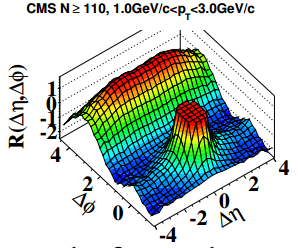
\includegraphics[width=0.47\linewidth]{figs/pp_high_multiplicity_ridge.PNG}
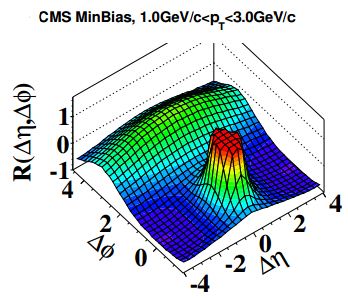
\includegraphics[width=0.47\linewidth]{figs/pp_correlation_function_min_bias.png}
\caption{ 2-D two-particle correlation function for $p+p$ collisions at \sqsn = 7 TeV for hadrons with 1.0 $<|p_T|<$ 3.0 GeV/c in high multiplicity events, with greater than 109 charged particles, and for any multiplicity of events are shown in the left and right panels, respectively\cite{Khachatryan2010}.}
\label{fig:pp_ridge_plot}
\end{center}
\end{figure}

What this discovery showed was that collectivity-like effects could be measured in small collisions systems for high-multiplicity events. Thus, $p+Pb$ at \sqsn = 5.02 TeV events were also analyzed to find flow and a nearside ridge was observed in 0-20\% central events. It became apparent over the course of making these measurements that the non-flow contribution to the signal would be much larger for p+A events then that of A+A events. A procedure to reduce the non-flow component in the flow measurement is demonstrated in Figure \ref{fig:pPb_ridge_subtraction}. The procedure measures the same two-particle correlation function for central and peripheral events, in this case 0-20\% central and 60-100\% central and then subtracts the central correlation function by the peripheral one. The assumption is that the level and shape of the non-flow is mostly consistent across centrality classes, whereas the flow is centrality dependent, such that there is virtually no flow in the peripheral correlation function. Thus, by subtracting the central correlation function by the peripheral, only the like components to both will be subtracted out, which are the non-flow components. As seen in panel three in Figure \ref{fig:pPb_ridge_subtraction}, the subtracted correlation function has no dominating jet peak at (0,0) and the nearside and awayside ridges are distinct and clear.

\begin{figure}[h!]
\begin{center}
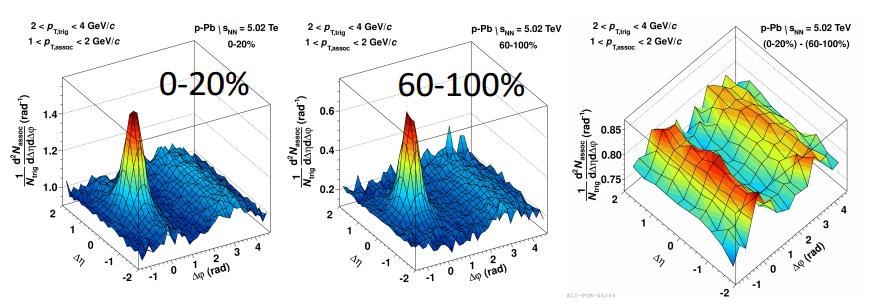
\includegraphics[width=0.85\linewidth]{figs/pPb_subtraction_correlation.PNG}
\caption{ 2-D two-particle dihadron correlation function for $p+Pb$ collisions for 0-20\% and 60-100\% centrality events as measured by the ALICE detector in the left and middle panel, respectively. The rightmost panel shows the subtraction of the left panel by the middle panel to remove background. [?]}
\label{fig:pPb_ridge_subtraction}
\end{center}
\end{figure}

\subsection{Mass Ordering in $v_2$}
A key observation in the determination of real collective flow is a mass ordering in the strength of the flow coefficients. The left panel of Figure \ref{fig:PbpPb_mass_ordering} depicts the observed mass ordering of particles in $Pb+Pb$ 10-20\% centrality events. In the low $p_T$ region of 0 - 2 GeV, there is an ordering in the magnitude of $v_2$ for hadrons: $\pi^{\pm}$ $>$ $K^{\pm}$ $>$ $p+pbar$ and so on for other heavier particles. This order is the opposite in which the hadrons are ordered by mass. The $\pi^{\pm}$ $v_2$ is the largest while the $\pi^{\pm}$ mass is the smallest. The mass ordering effect can be thought of as primarily a reduction in the $v_2$ for low $p_T$ heavy hadrons. Assuming an elliptic flow is present, the steep pressure gradients will efficiently modify the magnitude of $p_T$ for heavy hadrons more than for light hadrons, leading to a reduction in the number of heavy hadrons available at low $p_T$ to produce a low $p_T$ $v_2$ \cite{PhysRevC.77.044909}. Thus, the mass ordering observation is taken to be evidence that the system is creating a medium such that particles will flow in predictable ways.

\begin{figure}[h!]
\begin{center}
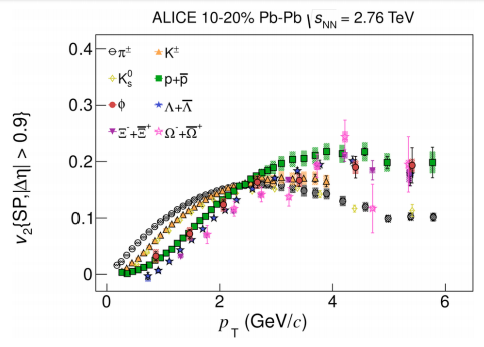
\includegraphics[width=0.48\linewidth]{figs/PbPb_v2_mass_ordering.PNG}
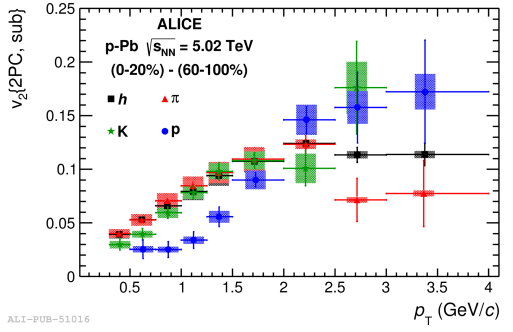
\includegraphics[width=0.48\linewidth]{figs/pPb_two_part_v2_mass_ordering.PNG}
\caption{$v_2(p_T)$ for different particles (see legend) in Pb-Pb \sqsn = 2.76 TeV 10-20\% events as measured by the ALICE detector. The $\Delta\eta$ gap at minimum is 0.9 units. The right plot shows the $v_2(p_T)$ for different particles (see legend) in p-Pb \sqsn = 5.02 TeV for 0-20\% events that were subtracted by peripheral 60-100\% events. The $v_2$ is extracted directly from the two particle correlation function shown in Figure \ref{fig:pPb_ridge_subtraction}. \textbf{add refs}}
\label{fig:PbpPb_mass_ordering}
\end{center}
\end{figure}

The right panel of Figure \ref{fig:PbpPb_mass_ordering} shows a similar plot to the left panel of that figure except for the system $p+Pb$ \sqsn = 5.02 TeV. As in the $Pb+Pb$ system, the $p+Pb$ dataset exhibits a the same mass ordering, as well as similar shapes of each $v_2(p_T)$ curve. Thus, the mass ordering effect that is observed in AA is also observed is small systems, such as pA. An important note for the result on the right panel is that a central minus peripheral subtraction was done, as demonstrated in Figure \ref{fig:pPb_ridge_subtraction}, whereas the result in the left panel needed no such peripheral subtraction. This means it is difficult to compare directly with the A+A result in magnitude, although the similarity of the ordering and the shape of the curves is enough of a comparison to indicate collectivity in the small system.

%\begin{figure}[h!]
%\begin{center}
%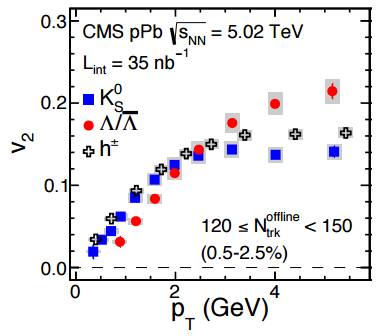
\includegraphics[width=0.55\linewidth]{figs/pBp_v2_mass_ordering.PNG}
%\caption{ CMS The correlation function for $p+p$ collisions at \sqsn = 7 TeV for hadrons with 1.0 $<|p_T|<$ 3.0 GeV/c in high multiplicity events with greater than 109 charged particle tracks were found \cite{Khachatryan2010}.}
%\label{fig:pp_ridge_plot}
%\end{center}
%\end{figure}

\subsection{Multi-Particle Cumulants and Fluctuations}
The effects of fluctuations in the elliptic flow measurement have been studied in small systems. In this context, fluctuations are effects which produce systematic correlations between particles from sources other than flow. Fluctuations can be thought of as correlations of a few particles in many events, rather than flow which is the correlations of many particles in a single event. Fluctuations are related to non-flow but are not identical. Fluctuations in the initial eccentricity can arise from fluctuations in the impact parameter within a centrality class of events and from fluctuations of the initial positions of the participant nucleons ~\cite{PhysRevC.80.014904}.

In order to better understand the effect of fluctuations in our small systems measurements, $v_2$ was measured in different ways such as, $v_2\{2\}$ and $v_2\{4\}$, which are given by equations \ref{eqn:v22} and \ref{eqn:v24}, respectively. The quantity $v_2\{2\}$ is the same as the two-particle correlation $v_2$, shown in Figure \ref{fig:PbpPb_mass_ordering}, while the quantity $v_2\{4\}$ is a four-particle correlation. This paper referenced here ~\cite{PhysRevC.80.014904}, defines a fluctuation term similar in form to standard deviation that is related to flow coefficients defined:

\begin{equation}
  \sigma_\nu^2 \equiv \left<\nu^2\right> - \left<\nu\right>^2,
\end{equation}
where $\nu$ is the flow coefficient relative to the participant plane. This fluctuation term is related to  $v_2\{2\}$ and $v_2\{4\}$ as 

\begin{equation}
\nu\{2\}^2 = \left<\nu^2\right> =  \left<\nu\right>^2 + \sigma_\nu^2,
\end{equation}
and
\begin{equation}
\nu\{4\}^2 = (2 \left<\nu^2\right>^2-\left<\nu^4\right>)^{1/2} \approx  \left<\nu\right>^2 -  \sigma_\nu^2.
\end{equation}
Thus, $v_2\{2\}$ measures the true elliptical flow plus fluctuations, whereas $v_2\{4\}$ measures the true elliptical flow minus fluctuations. By measuring both $v_2\{2\}$ and $v_2\{4\}$ for the same dataset, an estimate of the size of the fluctuations can be obtained. The difference between the two and four particle cumulants should be $\approx$ twice the size of the fluctuations.

Figure \ref{fig:pp_pPb_PbPb_cumulants} shows the measurement of multi-particle cumulants in $p+p$, $p+Pb$, and $Pb+Pb$ by the CMS collaboration at the LHC. A key part of this plot is noticing the significant difference between $v_2\{2\}$ and $v_2\{4\}$ in high multiplicity $p+Pb$ and $Pb+Pb$ events, indicating the presence of fluctuations. In the $p+Pb$ and $Pb+Pb$ there is an apparent multiplicity threshold, approximately around $N^{offline}_{trk}$ = 75, below which a class of peripheral events have a different kind of behavior than the high multiplicity events. 
%This is difference is interesting relative to the lack of splitting in $p+p$ events which could indicate the lack of fluctuations in that system. 
%paul romatchke ryan, 3 panel plot constituent quark initial condition pp 
% 6-8 and Lee Yang zeros N-body correlation, not a two body decay that correlations particles, not back to back jets correlated because tehy all feel the effects the initial geometry
\begin{figure}[!ht]
\begin{center}
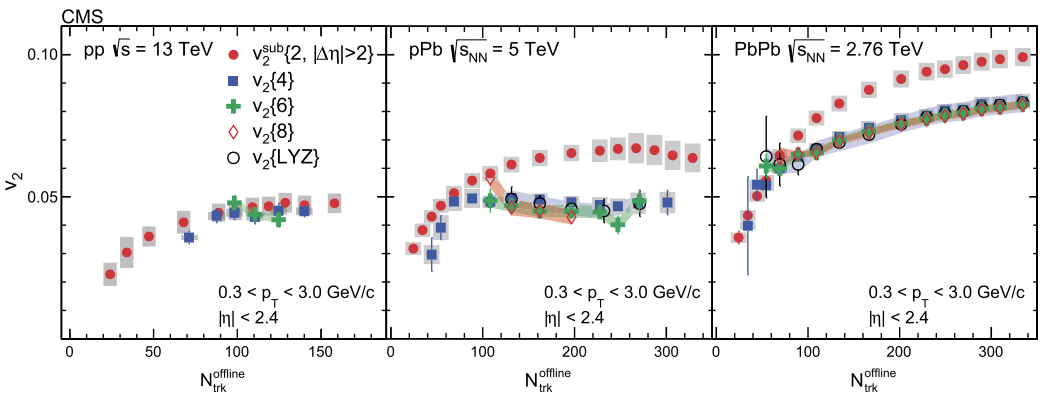
\includegraphics[width=0.95\linewidth]{figs/pp_pPb_PbPb_cumulants.PNG}
\caption{Elliptic flow measurements made using the 2nd, 4th, 6th, and 8th multi-particle cumulants, where the 2nd multi-particle is subtracted by peripheral events. Also the Lee Yang zero method non-flow elimination method is shown. These quantities are plotted vs the event multiplicity measured as $N^{offline}_{trk}$, which is the number of charged particle tracks observed during the offline analysis averaged over  $0.3 < p_T < 3.0$ GeV/c and over $|\eta| < 2.4$. The left panel is $v^{sub}_2\{2,|\Delta\eta|> 2\}$, $v_2\{4\}$, and $v_2\{6\}$ in $p+p$ collisions at $\sqrt{s}$ = 13 TeV. The middle panel $v^{sub}_2\{2,|\Delta\eta|> 2\}$, $v_2\{4\}$, $v_2\{6\}$, $v_2\{8\}$, and $v_2\{LYZ\}$ in $p+Pb$ at \sqsn = 5 TeV collisions. The right panel is  $v^{sub}_2\{2,|\Delta\eta|> 2\}$, $v_2\{4\}$, $v_2\{6\}$, $v_2\{8\}$, and $v_2\{LYZ\}$ in $Pb+Pb$ collisions at \sqsn = 2.76 TeV. The error bars correspond to the statistical uncertainties, while the shaded regions correspond to the systematic uncertainties~\cite{Khachatryan2017193}.}
\label{fig:pp_pPb_PbPb_cumulants}
\end{center}
\end{figure}

It is also interesting to note that for both systems, the $v_2\{4\}$, $v_2\{6\}$, $v_2\{8\}$, $v_2\{LYZ\}$ are in excellent agreement. The $v_2\{LYZ\}$ is $v_2$ measured taking into account the Lee-Yang zeros by removing all lower-order correlations. This excellent agreement indicates that $p+Pb$ is similar to $Pb+Pb$ in that it is a N-body correlation, not a two-body decay or back-to-back jets which produces correlations between particles. Although these types of processes are present, all particles feel the effects of the initial geometry.

\iffalse

\begin{figure}[h!]
\begin{center}
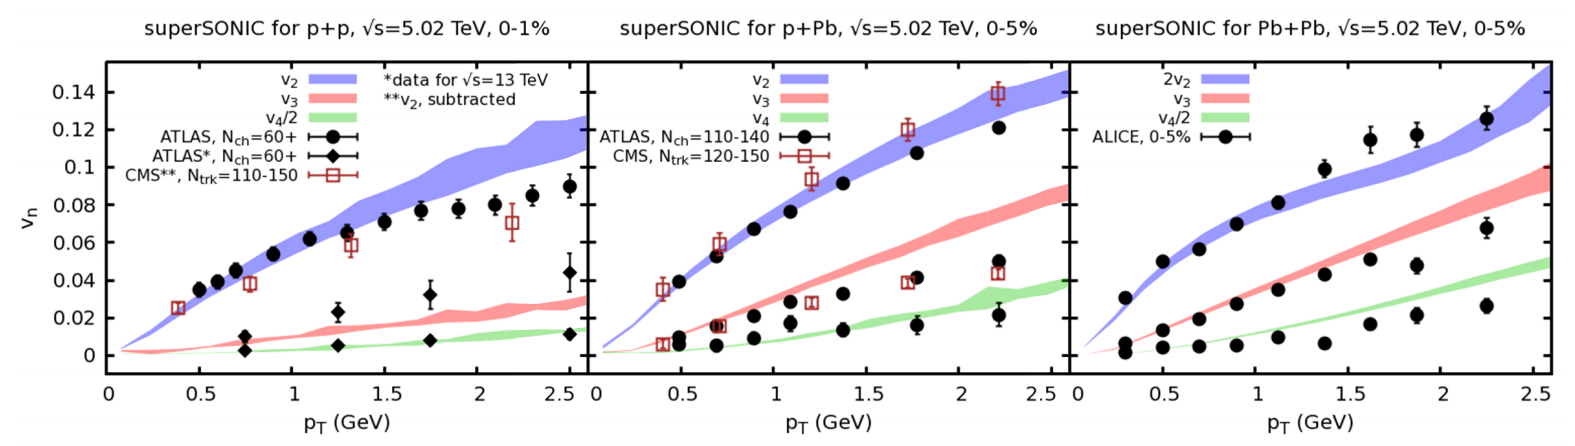
\includegraphics[width=0.75\linewidth]{figs/pp_ppb_pbpb_vn_supersonic.PNG}
\caption{ $v_2(p_T)$ for $d+Au$ and $\hau$ at \sqsn = 200 GeV 0-5\% centrality events for $\pi^{\pm}$ and $p+pbar$ separately. The boxes correspond to the systematic uncertainty. \textbf{add ref}}
\label{fig:lhc_flow_moments_sonic}
\end{center}
\end{figure}

\fi

\subsection{Measurements Made at RHIC}

Flow measurements in small systems have also be made at a lower energy accelerator, RHIC. Small collision systems, $d+Au$, $\hau$, and $p+Au$ at \sqsn = 200 GeV per nucleon were taken at RHIC in 2008, 2014, and 2015, respectively. The 2008 $d+Au$ dataset was intended to measure cold nuclear matter effects; however, RHIC experiments such as PHENIX had the capability to go back and measure $v_2(p_T)$. PHENIX was able to measure $v_2$ for $d+Au$ and for $\hau$ for the 0-5\% most central events, as shown in Figure \ref{fig:dhau_v2_v3}. A substantial $v_2$ is observed for both $d+Au$ and $\hau$ events with a $p_T$ dependence, which is similar to that seen in $p+Pb$ at the LHC. Instead of subtracting the non-flow component, as was done in Figure \ref{fig:pPb_ridge_subtraction}, the non-flow is incorporated as a systematic uncertainty. In addition to the $v_2$ measurement, a substantial $v_3$ is measured for the $\hau$ dataset. This measurement is significant because the observation of more than one flow indicates the system is exhibiting complex behavior. A single flow harmonic could be explained by a variety of causes, whereas two flow harmonics from the same system narrow the range of possible explanations.

\begin{figure}[h!]
\begin{center}
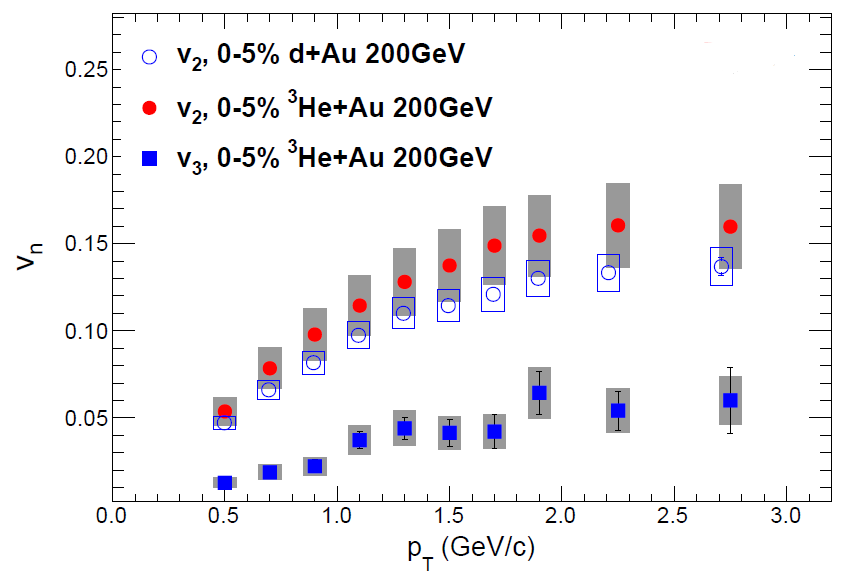
\includegraphics[width=0.75\linewidth]{figs/hedau_v2_v3.PNG}
\caption{ $v_n(p_T)$ measured for $d+Au$ and $\hau$ at \sqsn = 200 GeV for 0-5\% central events. $v_2$ was measured for both systems and $v_3$ was measured for $\hau$. The grey boxes correspond to systematic uncertainties. \textbf{add ref}}
\label{fig:dhau_v2_v3}
\end{center}
\end{figure}

In addition to measuring the $v_2(p_T)$ for all hadrons, $v_2$ has been measured for $\pi^{\pm}$ and $p+pbar$, as seen in Figure \ref{fig:dhau_mass_ordering}. A very similar mass ordering in $v_2(p_T)$ for different hadrons that was observed for $p+Pb$ at \sqsn = 5.02 TeV  in Figure \ref{fig:PbpPb_mass_ordering}, was also observed for $d+Au$ and $\hau$ at \sqsn =  200 GeV. In the low $p_T$ region, $ p_T <$ 1.5 GeV, the $v_2$ for $\pi^{\pm}$ is greater than the $v_2$ for $p+pbar$. An interesting note here is that the low $p_T$ region only goes up to 1.5 GeV/c, whereas the $p+Pb$ dataset shows a low $p_T$ mass ordering region of up to 2 GeV/c. The reason for this is probably due to the difference in center of mass energy.

\begin{figure}[h!]
\begin{center}
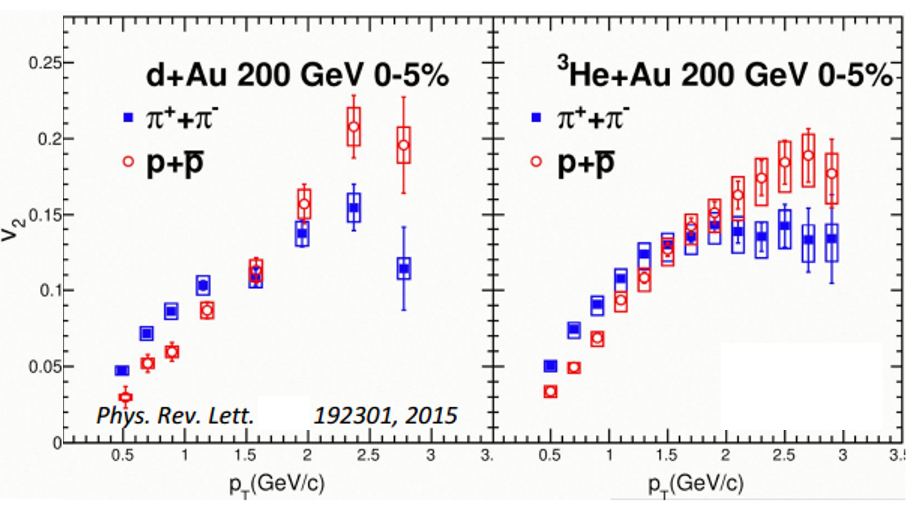
\includegraphics[width=0.75\linewidth]{figs/dhau_mass_ordering_phenix.PNG}
\caption{ $v_2(p_T)$ for $d+Au$ and $\hau$ at \sqsn = 200 GeV 0-5\% centrality events for $\pi^{\pm}$ and $p+pbar$ separately. The boxes correspond to the systematic uncertainty. \textbf{add ref}}
\label{fig:dhau_mass_ordering}
\end{center}
\end{figure}

It is necessary to note that throughout all of these measurements in small systems, a skepticism to the interpretation that the measurements are hydrodynamic flow has persisted. There are alternative explanations to the apparent flow measured in small systems which do not involve the creation of a medium. In order to further the discussion on the distinction between a medium and a non-medium explanation, three different small collision systems, each with unique initial conditions, were run at RHIC. Those three systems are d+Au, He+Au, and finally p+Au, with intrinsic  elliptical, triangular, and circular geometric initial conditions. The constraints that a set of measurements from all three systems would place upon explanatory models would help distinguish which theory best describes small systems. This thesis is the completion of that set of three measurements, by measuring $v_2$ in the p+Au dataset.

%However, evidence of collectivity has recently been observed at RHIC in p+Au collisions at $\sqrt{s_{NN}}$ = 200 GeV in the most central collisions ~\cite{PhysRevLett.115.142301}. Although, the $p_T$ dependent $v_N$ has been measured, what has not been measured in these small systems is the degree to which $v_N$ changes a function of rapidity. This is a particularly interesting measurement to make in an asymmetric collision system such as p+Au.

%Recent analyses of d+Au and HeAu collisions at $\sqrt{n}$ = 200 GeV~\cite{PhysRevLett.111.212301,Adare:2014keg,Adare:2015ctn,Adamczyk:2014fcx} at the Relativistic Heavy-Ion Collider (RHIC), and p+Pb at $\sqrt{n}$ = 5.02 TeV, and $p+p$ collisions at $\sqrt{n}$ = 2.76, 5.02, 7, and 13 TeV~\cite{alice_long_2013,atlas_observation_2012,cms_observation_2012,Khachatryan:2015lva,Aad:2015gqa,Khachatryan:2010gv,Khachatryan:2016txc} at the Large Hadron Collider (LHC) have demonstrated the existence of the same kind of azimuthal anisotropy signals commonly interpreted as evidence of collective behavior in larger systems. Notably, a feature known as \textit{the ridge} has been observed, consisting of a near-side (i.e., at small relative azimuth) enhancement in the long-range (i.e., at large relative pseudorapidity) azimuthal two-particle correlation. From these correlations, substantial elliptic ($v_2$), and triangular ($v_3$) flow coefficients have been measured in these systems.

%\iffalse



%\fi